\documentclass{llncs}

\usepackage[T1]{fontenc}
% T1 fonts will be used to generate the final print and online PDFs,
% so please use T1 fonts in your manuscript whenever possible.
% Other font encondings may result in incorrect characters.
\usepackage{graphicx}
\usepackage{hyperref}
\usepackage{comment}
\usepackage[inline]{enumitem}

\newcommand{\lab}[1]{\textsf{#1}}
\newcommand{\blab}[1]{\lab{\bfseries #1}}
\newcommand{\ilab}[1]{\lab{\itshape #1}}

%%%%%% To display ORCID Logo with link, Please add below definition and copy the ORCID_Color.eps in the manuscript package %%%%%
\makeatletter
	\def\@citecolor{blue}%
	\def\@urlcolor{blue}%
	\def\@linkcolor{blue}%
	\def\UrlFont{\rmfamily}
	\def\orcidID#1{\smash{\href{http://orcid.org/#1}{\protect\raisebox{-1.25pt}{\protect
\includegraphics{ORCID_Color.eps}}}}}
\makeatother

\begin{document}

\title{Experimenting with Reaction Systems using Graph Tansformation}
\author{Roberto Bruni\inst{1}\orcidID{0000-0002-7771-4154}  \and 
            Arend Rensink\inst{2}\orcidID{0000-0002-1714-6319}}

\institute{
University of Pisa, Italy,
\email{roberto.bruni@unipi.it} \and
University of Twente, Netherlands,
\email{arend.rensink@utwente.nl}}


\maketitle
\begin{comment}
\begin{abstract}
We explore the capabilities of GROOVE, a state-of-the-art toolset based on graph transformation systems, to perform reachability and causal analysis of Reaction Systems.
Our results are still preliminary, but encouraging, as in the presence of large state spaces GROOVE outperforms available applications by halving the analysis time of both reachability and causal analyses.
From the point of view of GROOVE, the implementation of Reaction Systems provided some interesting insights on the most convenient way to model certain computational requirements through negative and nested application conditions.
\end{abstract}
\end{comment}

We explore the capabilities of  a state-of-the-art toolset based on graph transformation  to perform reachability and causal analysis of Reaction Systems.

Reaction systems (RS)~\cite{DBLP:journals/fuin/EhrenfeuchtR07} are a computational model inspired by the functioning of biochemical reactions within living cells. 
%The primary motivation behind RS is to provide a simple yet expressive model for understanding and analyzing processes in natural and artificial systems.
RS focus on the interaction of entities through a set of reactions. 
Each reaction relies on some reactants, inhibitors, and products to mimic two fundamental mechanisms found in nature: facilitation and inhibition.
%Facilitation means that a reaction can occur only if all of its reactants are present, while inhibition means that a reaction cannot occur if any of its inhibitors is present. 
At each time instant, the next state of the system is determined by the products of all enabled reactions plus some additional entities that are possibly provided by environment.
Unlike traditional models of concurrency, like Petri nets, the theory of RS is based on three principles: \emph{no permanency}, any entity vanishes unless it is sustained by a reaction; \emph{no competition}, an entity is either available for all reactions, or it is not available at all; and \emph{no counting}, the exact concentration level of available entities is ignored.
Recent applications concerned, e.g., with the efficacy of medical treatments for comorbidities and with the selection of the best environment to achieve some desired phenomena, led to experiment with environments that exhibit nondeterministic and recursive behaviour.
Then, performing reachability and causal analysis required the exploration of large state spaces for which the available prototype tool~\cite{DBLP:journals/tcs/BrodoBF21} struggled in terms of  memory consumption and response time.
 
Graph Transformation (GT)~\cite{DBLP:series/eatcs/EhrigEPT06,DBLP:books/sp/HeckelT20} is a modelling technique that is widely applicable in problem domains where the objects of study have an inherent graphical structure, and the task at hand is to study their properties and evolution. Besides the graphs themselves, the core concept is that of a (transformation) \emph{rule} capturing a particular change to such a graph. Rules can be used, for instance, to describe the change of a system over time, but can also be instrumental in composing and decomposing graphs and so exposing structural properties.

Importantly for the utility of the technique, there are a number of (academic) tools supporting its use. The research described here crucially relies on \href{https://groove.cs.utwente.nl}{GROOVE}~\cite{DBLP:journals/sttt/GhamarianMRZZ12}, one of the most prominent tools in this area, which was designed precisely to enable GT-based system analysis of the kind described above. Two features of GROOVE that are essential for the purpose of this research are
\begin{enumerate*}[label=\emph{(\roman*)}]
\item nested (i.e., quantified) rules, which capture simultaneous changes in all neighbourhoods that satisfy certain application conditions, rather than only locally in one such neighbourhood at a time; and
\item exploration of the set of reachable graphs (under the given rules) using various strategies.
\end{enumerate*}

We are in the process of investigating how GT can help in addressing the analysis questions in Reaction Systems. For this purpose, we encode a given RS as a single graph, upon which a small number of (fixed) rules operate to simulate the correct semantics. The core rule describes the simultaneous firing of all \blab{Reaction}s of which no \lab{inhibitor}s and all \lab{reactant}s are present; the firing results in the presence of all \lab{product}s. Simultaneously, all currently present \blab{Entity}s are removed. In GROOVE syntax, this looks as follows:

\begin{center}
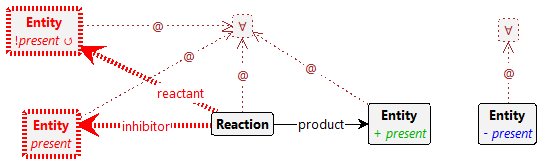
\includegraphics[scale=.49]{react}
\end{center}

To parse this, note that (in the GROOVE rule syntax) the red structure must be absent for the rule to apply; moreover, green labels are added and blue ones deleted upon rule application. The \ilab{present} flag signals whether an \blab{Entity} is considered to be currently present; hence, creating or deleting that flag comes down to creating or deleting the \blab{Entity}. The $\forall$-nodes impose the desired quantification, causing a single application of this rule to model the firing of all enabled \blab{Reaction}s, even if there are thousands of them.

Our model also supports environments that inject \blab{Entity}s in a controlled manner. This is achieved through a second rule, not shown here. A configuration is reachable if it can be constructed by the alternating application of both rules.

\medskip\noindent
Our first results are encouraging: GROOVE seems capable to explore larger Reaction Systems 
%is well beyond what other tools have been able to achieve, 
by halving the analysis time of both reachability and causal analyses.
More precisely, we are able to find a trace towards unwanted patterns (if they exist) among millions of reachable configurations using different heuristics; then, we can also prune the trace to extract a graphical representation of the causal history of that entities, at least as far as reactants are concerned.

% ---- Bibliography ----
%
% BibTeX users should specify bibliography style 'splncs04'.
% References will then be sorted and formatted in the correct style.
%
\bibliographystyle{splncs04}
\bibliography{references}
%

\end{document}
